% sIVM: certified reuse for LLM-computed table columns.
% Target: PVLDB Vol. 20 (rolling deadline the 1st of each month; mandatory
% abstract the 25th of the prior month) -> VLDB 2027.
% Format: the official PVLDB template (acmart.cls v2.19 pinned by the
% VLDB-Template bundle + pvldb.sty), fetched from
% https://github.com/vldbproceedings/VLDB-Template. Deviating from it is
% grounds for desk rejection, so acmart.cls/pvldb.sty/ACM-Reference-Format.bst
% are vendored here unmodified rather than taken from a local TeX install.
% The arXiv source package omits pvldb.sty: it is not loaded in arXiv
% mode (see the \ifarxiv toggle below).
% Limit: 12 pages excluding references (appendices and acknowledgements count).
% Review model: single-blind, so author names and affiliations stay on page 1.
\documentclass[sigconf, nonacm]{acmart}

%% Build mode. \arxivtrue produces the arXiv preprint; \arxivfalse the PVLDB
%% submission. The PVLDB Reference Format block and the CC BY-NC-ND footer
%% assert a VLDB Endowment publication that has not happened, so neither may
%% appear on the preprint; pvldb.sty is therefore not loaded in arXiv mode.
\newif\ifarxiv
\arxivtrue

\ifarxiv\else
%%% do not modify the following VLDB block %%
%%% VLDB block start %%%
\usepackage{pvldb}% VLDB/PVLDB formatting overrides, see pvldb.sty for details.
                      % Do not remove -- required for consistent proceedings
                      % formatting across all VLDB submissions.
%%% VLDB block end %%%

%% Set per paper. Volume/issue/year defaults live in pvldb.sty.
\renewcommand\vldbdoi{XX.XX/XXX.XX}
\renewcommand\vldbpages{XXX-XXX}
%% Left empty deliberately: set to the artifact archive URL when it is public.
%% PVLDB requires a public archival URL at submission.
\renewcommand\vldbavailabilityurl{}
\fi

\usepackage{amsmath,amssymb}
\usepackage{booktabs}
\usepackage{needspace}% a heading must not be stranded at the foot of a column
\newcommand{\keepheading}{\needspace{6\baselineskip}}% before a section heading
\newcommand{\keeprunin}{\needspace{4\baselineskip}}% before a run-in heading
\usepackage{array}% ragged-right paragraph columns in the prose tables
\usepackage{algorithm}
\usepackage{algorithmic}
\usepackage{pgfplots}
\pgfplotsset{compat=1.18}
\usetikzlibrary{arrows.meta, positioning, calc}
% GENERATED. Do not edit.
\newcommand{\frontierplots}{\addplot+[error bars/.cd, y dir=both, y explicit] coordinates { (0.02,0.0) +- (0,0.0) (0.05,38.6) +- (0,29.5) (0.1,82.6) +- (0,9.8) (0.2,88.1) +- (0,0.8) }; \addlegendentry{SO formatting-only} \addplot+[error bars/.cd, y dir=both, y explicit] coordinates { (0.02,0.0) +- (0,0.0) (0.05,0.0) +- (0,0.0) (0.1,55.6) +- (0,29.0) (0.2,87.4) +- (0,3.2) }; \addlegendentry{SO synonym rewording} \addplot+[error bars/.cd, y dir=both, y explicit] coordinates { (0.02,0.0) +- (0,0.0) (0.05,1.0) +- (0,8.8) (0.1,66.3) +- (0,25.1) (0.2,86.6) +- (0,3.1) }; \addlegendentry{SO scope widening} \addplot+[error bars/.cd, y dir=both, y explicit] coordinates { (0.02,0.0) +- (0,0.0) (0.05,0.0) +- (0,0.0) (0.1,8.4) +- (0,10.6) (0.2,52.1) +- (0,10.1) }; \addlegendentry{Djinni formatting-only} \addplot+[error bars/.cd, y dir=both, y explicit] coordinates { (0.02,0.0) +- (0,0.0) (0.05,0.0) +- (0,0.0) (0.1,14.4) +- (0,11.0) (0.2,48.6) +- (0,10.4) }; \addlegendentry{Djinni criteria change}}
\newcommand{\powerplots}{\addplot coordinates { (0,100.0) (0.005,99.9) (0.01,98.9) (0.02,88.7) (0.04,22.8) (0.05,5.5) (0.0525,3.5) (0.055,2.8) (0.0625,0.9) (0.08,0.2) (0.15,0.0) }; \addlegendentry{$n_j{=}600$} \addplot coordinates { (0,100.0) (0.005,99.9) (0.01,98.9) (0.02,92.0) (0.04,48.4) (0.05,9.8) (0.0525,6.2) (0.055,3.0) (0.0625,0.8) (0.08,0.1) (0.15,0.0) }; \addlegendentry{$n_j{=}1{,}800$} \addplot coordinates { (0,100.0) (0.005,99.8) (0.01,98.9) (0.02,92.5) (0.04,28.9) (0.05,2.9) (0.0525,1.1) (0.055,0.7) (0.0625,0.0) (0.08,0.0) (0.15,0.0) }; \addlegendentry{$n_j{=}5{,}000$}}

% GENERATED by scripts/experiments/gen-paper-assets.ts. Do not edit.
% Every number cited in prose is defined here from result artifacts.
\newcommand{\floorBool}{5.0\%}
\newcommand{\editFlipFreshBoth}{7.2\%}
\newcommand{\floorTrueStratum}{24.1\%}
\newcommand{\floorFalseStratum}{3.1\%}
\newcommand{\floorTrueCi}{[19.6, 28.8]}
\newcommand{\floorFalseCi}{[2.5, 3.7]}
\newcommand{\floorBoolVote}{6.30\%}
\newcommand{\floorBoolStored}{6.0\%}
\newcommand{\labelChurn}{4.8\%}
\newcommand{\flipInstrumentGapRows}{7}
\newcommand{\floorSelect}{6.5\%}
\newcommand{\floorDefaultT}{9.5\%}
\newcommand{\floorTzeroProbe}{3.0\%}
\newcommand{\flipSoFormatting}{6.3\%}
\newcommand{\flipSoSynonym}{8.90\%}
\newcommand{\flipSoWidening}{9.45\%}
\newcommand{\flipDjFormatting}{12.30\%}
\newcommand{\flipDjCriteria}{12.45\%}
\newcommand{\benchN}{2{,}000}
\newcommand{\benchSavings}{82.6\%}
\newcommand{\benchSavingsMain}{86.2\%}
\newcommand{\benchSavingsPi}{[82, 86]}
\newcommand{\benchRealizedCi}{[2.6, 4.3]}
\newcommand{\bootB}{1{,}000}
\newcommand{\benchRealized}{3.20\%}
\newcommand{\benchOracleTight}{765}
\newcommand{\benchOracleMain}{135}
\newcommand{\frontierA}{82.6\%}
\newcommand{\frontierB}{63.6\%}
\newcommand{\frontierC}{0.1\%}
\newcommand{\edgeCertRate}{0.8\%}
\newcommand{\edgeExceed}{100.0\%}
\newcommand{\sampleFracLo}{7\%}
\newcommand{\sampleFracHi}{81\%}
\newcommand{\benchOracleMean}{208}
\newcommand{\benchOracleMedian}{225}
\newcommand{\benchOracleRange}{135--405}
\newcommand{\benchOracleTightMean}{568}
\newcommand{\benchOracleTightRange}{90--765}
\newcommand{\benchOracleTightMedian}{405}
\newcommand{\reuseSetSavingsMain}{81.4\%}
\newcommand{\reuseSetSavingsTight}{8.1\%}
\newcommand{\reuseSetCertTight}{11.7\%}
\newcommand{\reuseSetDjCertMax}{0.8\%}
\newcommand{\tableConfigs}{20}
\newcommand{\certifyingConfigs}{9}
\newcommand{\ablationSavings}{61.4\%}
\newcommand{\ablationTotal}{40}
\newcommand{\ablationBetter}{1}
\newcommand{\ablationWorse}{16}
\newcommand{\aucVcacheF}{0.468}
\newcommand{\aucVcacheW}{0.499}
\newcommand{\aucInterF}{0.408}
\newcommand{\aucInterW}{0.669}
\newcommand{\simLo}{0.96}
\newcommand{\simHi}{0.99}
\newcommand{\aggFsavings}{91.0\%}
\newcommand{\aggFrealized}{5.99\%}
\newcommand{\aggFsubgroup}{36.1\%}
\newcommand{\aggWsubgroup}{44.1\%}
\newcommand{\aggWsavings}{64.0\%}
\newcommand{\aggWrealized}{9.45\%}
\newcommand{\aggTightCertF}{certifies}
\newcommand{\aggFtSavings}{28.0\%}
\newcommand{\aggFtRealized}{6.07\%}
\newcommand{\aggFtSubgroup}{45.2\%}
\newcommand{\aggTightCertW}{refuses}
\newcommand{\tauFmid}{100\%}
\newcommand{\tauFhi}{10.4\%}
\newcommand{\tauFerrLo}{4.8\%}
\newcommand{\tauFerrHi}{6.3\%}
\newcommand{\tauWmid}{99.9\%}
\newcommand{\tauWhi}{8.2\%}
\newcommand{\tauWerrLo}{8.0\%}
\newcommand{\tauWerrHi}{9.9\%}
\newcommand{\minoritySingle}{37.1\%}
\newcommand{\minorityVote}{24.7\%}
\newcommand{\minorityNoise}{20.4\%}
\newcommand{\calTrials}{396{,}000}
\newcommand{\calConfigs}{198}
\newcommand{\bThreeReuseW}{84.2\%}
\newcommand{\minZeroFlipRealized}{360}
\newcommand{\calPRange}{[0, 0.25]}
\newcommand{\calTightNulls}{54}
\newcommand{\calTightWorstCert}{0.0\%}
\newcommand{\calAlphaGrid}{0.05, 0.1, 0.2}
\newcommand{\calWorstReuseMetric}{33.3\%}
\newcommand{\calWorstP}{0.04}
\newcommand{\calWorstAlpha}{0.05}
\newcommand{\calWorstCertRate}{0.45\%}
\newcommand{\deployN}{89{,}184}
\newcommand{\deployOracle}{225}
\newcommand{\deployReused}{81{,}289}
\newcommand{\deployRecompute}{7{,}670}
\newcommand{\deploySavings}{91.1\%}
\newcommand{\deployRealized}{3.01\%}
\newcommand{\deployOverlap}{2{,}159}
\newcommand{\deployReplayMs}{4{,}257}
\newcommand{\deployTrueStratum}{7{,}715}
\newcommand{\deployCeiling}{91.3\%}
\newcommand{\deployOracleTight}{765}
\newcommand{\deploySavingsTight}{90.5\%}
\newcommand{\deployStamped}{79{,}130}
\newcommand{\deployUnstamped}{2{,}159}
\newcommand{\perCellCost}{\$0.00012}
\newcommand{\deployMatCost}{\$9.31}
\newcommand{\deployMatCells}{78{,}956}
\newcommand{\deployFreeRows}{10{,}228}
\newcommand{\deployMatHours}{7.4}
\newcommand{\deployConcurrency}{32}
\newcommand{\deployMaintCells}{7{,}895}
\newcommand{\deployMaintCost}{\$0.93}
\newcommand{\deployMaintMinutes}{43}
\newcommand{\deployAuditReleased}{1{,}807}
\newcommand{\deployAuditReleasedErr}{3.21\%}
\newcommand{\hhBudget}{135}
\newcommand{\hhSivmReused}{1{,}724}
\newcommand{\hhSivmErr}{3.36\%}
\newcommand{\hhSupgReused}{1{,}865}
\newcommand{\hhSupgErr}{6.54\%}
\newcommand{\hhSupgTrueRows}{180}
\newcommand{\hhSivmPerTest}{\delta/12}
\newcommand{\hhValuePerTest}{\delta/3}
\newcommand{\hhSivmErrW}{5.49\%}
\newcommand{\hhSupgErrW}{9.69\%}
\newcommand{\hhSupgTrueRowsW}{185}
\newcommand{\hhSivmReusedW}{1{,}621}
\newcommand{\hhSupgReusedW}{1{,}775}
\newcommand{\hhSivmReusedFrac}{86.2\%}
\newcommand{\hhSupgReusedFrac}{93.3\%}
\newcommand{\hhSivmReusedFracW}{81.0\%}
\newcommand{\hhSupgReusedFracW}{88.8\%}
\newcommand{\hhSupgSelFrac}{100.0\%}
\newcommand{\hhSupgSelFracW}{100.0\%}
\newcommand{\deployWorLoose}{0.230}
\newcommand{\deployLooseSampled}{180}
\newcommand{\deployLooseFlips}{5}
\newcommand{\deployWorLooseClears}{does not clear}
\newcommand{\deployWorTight}{0.099}
\newcommand{\deployTightSampled}{720}
\newcommand{\deployTightFlips}{25}
\newcommand{\deployWorTightClears}{clears}
\newcommand{\deployFalseStratum}{81{,}469}
\newcommand{\altModelName}{openai/gpt-5-nano}
\newcommand{\altModelFloor}{36.6\%}
\newcommand{\altModelEditFlip}{40.2\%}
\newcommand{\altModelN}{500}
\newcommand{\minZeroFlipSample}{$n^{*}{=}257$}
\newcommand{\corpusSO}{89{,}184}
\newcommand{\corpusDjinni}{210{,}250}
\newcommand{\labeledCells}{32{,}000}
\newcommand{\wideningTrueFlip}{45.7\%}
\newcommand{\wideningTrueCi}{[39.0, 52.7]}
\newcommand{\wideningTrueN}{199}
\newcommand{\boundConfigsTotal}{20}
\newcommand{\boundEbConfigs}{7}
\newcommand{\boundBetConfigs}{9}
\newcommand{\boundWorConfigs}{7}
\newcommand{\boundEbSavings}{18.5\%}
\newcommand{\boundBetSavings}{29.1\%}
\newcommand{\boundEbOracle}{11{,}515}
\newcommand{\boundBetOracle}{7{,}616}
\newcommand{\boundEbAtN}{0.144}
\newcommand{\boundBetAtN}{0.065}
\newcommand{\boundWorAtN}{0.317}
\newcommand{\boundWorSameLook}{3}
\newcommand{\boundWorLater}{4}
\newcommand{\boundWorLost}{0}
\newcommand{\boundWorExtra}{0}
\newcommand{\boundWorOracle}{12{,}325}
\newcommand{\boundWorSavings}{16.4\%}
\newcommand{\boundGapEbSavings}{18.1\%}
\newcommand{\boundGapBetSavings}{72.0\%}
\newcommand{\boundGapEbOracle}{1{,}485}
\newcommand{\boundGapBetOracle}{405}
\newcommand{\boundCalTrials}{72{,}000}
\newcommand{\boundBetNullWorst}{2.5\%}
\newcommand{\boundBetNullsOver}{0}
\newcommand{\boundNullConfigs}{18}
\newcommand{\boundEbCleanSample}{360}
\newcommand{\boundBetCleanSample}{180}
\newcommand{\totalSpend}{\$11.56}
\newcommand{\ledgerStart}{4 August 2026}
\newcommand{\ledgerEnd}{5 August 2026}
\newcommand{\famRunDate}{15 August 2026}
\newcommand{\totalCells}{98{,}496}
\newcommand{\offLedgerCells}{38{,}416}
\newcommand{\famGeminiFloor}{4.9\%}
\newcommand{\famGeminiFmt}{25.4\%}
\newcommand{\famGeminiSyn}{31.5\%}
\newcommand{\famGeminiN}{2{,}000}
\newcommand{\famGeminiFmtTrueStratum}{28.7\%}
\newcommand{\famGeminiFmtFalseStratum}{24.6\%}
\newcommand{\famGeminiFmtToFalseShare}{24.6\%}
\newcommand{\famGeminiCachedTrueShare}{21.8\%}
\newcommand{\famGeminiCaseOnlyFlip}{11.0\%}
\newcommand{\famGeminiSpaceOnlyFlip}{23.2\%}
\newcommand{\famGeminiCaseOnlyCert}{60.2\% @ 405}
\newcommand{\famGeminiSpaceOnlyCert}{refused (90)}
\newcommand{\famGeminiThreeFloor}{0.4\%}
\newcommand{\famGeminiThreeFmt}{5.8\%}
\newcommand{\famGeminiThreeN}{500}
\newcommand{\famGlmFloor}{10.3\%}
\newcommand{\famGlmFmt}{25.0\%}
\newcommand{\famGlmSyn}{31.3\%}
\newcommand{\famGlmN}{2{,}000}
\newcommand{\famGlmFmtTrueStratum}{27.0\%}
\newcommand{\famGlmFmtFalseStratum}{17.0\%}
\newcommand{\famGlmFmtToFalseShare}{86.4\%}
\newcommand{\famGlmCachedTrueShare}{80.0\%}
\newcommand{\famQwenFloor}{5.8\%}
\newcommand{\famQwenFmt}{14.6\%}
\newcommand{\famQwenN}{500}
\newcommand{\famCount}{4}
\newcommand{\famCertifying}{3}
\newcommand{\famFloorLo}{0.4\%}
\newcommand{\famFloorHi}{10.3\%}


%% Two-column measure is narrow and the prose carries long \texttt{} paths
%% and identifiers; let TeX stretch the line rather than run into the gutter.
\setlength{\emergencystretch}{2em}

%% acmart already provides theorem/lemma/proof; only assumption is ours.
\theoremstyle{acmdefinition}
\newtheorem{assumption}{Assumption}
\newcommand{\sivm}{\textsc{sIVM}}
%% Venue dialect hooks shared with body.tex (the IEEE shell defines its own).
\newcommand{\secref}[1]{\S\ref{#1}}
\newcommand{\figref}[1]{Figure~\ref{#1}}
\newcommand{\paperroot}{.}
\newcommand{\venueappendix}{\appendix}
\newcommand{\venueroadmap}{}

\begin{document}

%% No short-title argument: \vldbtitle defaults to \shorttitle, so a
%% bracketed short form would make the PVLDB Reference Format block on page 1
%% print a citation string with the subtitle dropped.
\title{Reuse, but Verify: Certified Maintenance of LLM-Computed Table
Cells under Prompt Edits}

\author{Arjun Lohan}
\affiliation{%
  \institution{Independent Researcher}
  \country{United States}
}
\email{arjunlohan7@gmail.com}
\email{lohan@usc.edu}

\begin{abstract}
AI-native tables let users define columns in natural language: each cell
is computed by a language model from a versioned prompt over its row.
When the prompt is edited, deployed systems face a choice:
recompute every cell, which is expensive and rate-limited, or silently
reuse stale ones, which incurs unbounded error. We present \sivm{}, a
maintenance layer that certifies which cached cells may be reused after
a prompt edit, bounding the false-reuse rate of each certified stratum
by a user budget $\alpha$ with probability at least $1-\delta$.
\sivm{} freezes cached-value strata, samples adaptively on a doubling
look schedule, and bounds each stratum's flip rate with an exact
finite-population confidence bound; a strict mode certifies at a
deflated threshold to bound the error of the reused cells alone. We
also establish an impossibility floor for this estimand: a model's rate of disagreement
with itself under the unedited prompt floors the certifiable
budget. On two
public corpora (\corpusSO\ Stack Overflow developer profiles;
\corpusDjinni\ Djinni candidate CVs) with \labeledCells\ labeled cells
and a production table system, a formatting-only edit certifies \benchSavingsMain\ call savings at $\alpha{=}0.2$ with \benchRealized\
realized false-reuse, and at deployment scale \deployOracle\ oracle
calls certify reuse of \deployReused\ of \deployN\ cells. Across
\calTrials\ calibration runs with planted flip rates, unsafe
certificates occur in at most \calUnsafeWorst\ of runs in any
configuration, against a nominal per-stratum budget of
\calNominalDelta. A second certification \driftDaysLater\ days later,
against the same cache, measured provider-side model drift as a higher
flip rate and re-certified the same budgets, the tighter one a look deeper than on
the August draws. Certification reproduces
on \famCertCount\ of \famCount\ further model families, while which edits
are benign varies by family. We release the system under a
source-available noncommercial license, with the labels and a benchmark
of versioned prompt-edit pairs.
\end{abstract}

\maketitle

\ifarxiv
%% Preprint identity: the DOI is reserved on Zenodo so it can be embedded
%% in the file before upload (Zenodo locks files after publishing).
\begingroup
\renewcommand\thefootnote{}\footnote{\noindent Preprint. This version is
archived at
\href{https://doi.org/10.5281/zenodo.21833641}{doi:10.5281/zenodo.21833641}.}%
\addtocounter{footnote}{-1}\endgroup
\else
%%% do not modify the following VLDB block %%
%%% VLDB block start %%%
\vldbtopmatter
%%% VLDB block end %%%
\fi

%% Shared paper body: Introduction through Availability. Included by two
%% venue shells that own everything above \section{Introduction}:
%%   main.tex       -- acmart: arXiv preprint / PVLDB (\ifarxiv toggle)
%%   ieee/main.tex  -- ieeeaccess: IEEE Access submission
%% Each shell must define: \secref (section cross-reference dialect),
%% \paperroot (relative path to this directory), \sivm, and the
%% theorem/assumption environments. Numbers remain macro-cited; the guards in
%% scripts/check-paper-numbers.ts scan this file plus both shells.
\section{Introduction}
\label{sec:intro}

Interactive AI tables (data-enrichment sheets, recruiter search
tables, spreadsheet copilots) turn a natural-language prompt into a
\emph{materialized view}: a column $V = (\pi, M, \theta)$ with prompt
$\pi$, model $M$, and pinned decode parameters $\theta$, materialized as
cells $c_i = f_V(r_i)$ over rows $r_1,\dots,r_n$. These views are edited
constantly: users iterate on prompts the way they iterate on
spreadsheet formulas. Every edit invalidates the cache by construction,
and today's systems invalidate it wholesale: an edit to an \corpusSO-row
column triggers \corpusSO\ fresh model calls, or the user silently keeps
stale values with no bound on how wrong they are.

Recent semantic data systems bound the error of \emph{one-shot} query
execution against a gold model (cascades, semantic operators, approximate
processing with guarantees), and verified semantic caches bound reuse
under a \emph{fixed} definition. Neither answers the maintenance
question an interactive table actually poses: \emph{after this specific
edit $\pi \to \pi'$, which cached cells are still valid, and with what
guarantee?}

\subsection{Why intuition fails here}
Three measurements reframe the problem (\secref{sec:experiments}).
First, large language model (LLM) cells are stochastic even at temperature zero: the same
prompt on the same row disagrees with itself \floorBool\ of the time on
our boolean workload (within-version draw pairs on $n{=}\benchN$; an
earlier $n{=}200$ two-draw probe read \floorTzeroProbe) and
\floorDefaultT\ at default temperature, so ``did the edit change this
cell?'' is only meaningful relative to a noise floor. Second, edit
direction is not monotone: under a strictly scope-\emph{widening} edit,
\wideningTrueFlip\ of
cached-TRUE cells flipped (\wideningTrueCi\ over \wideningTrueN\
such cells), refuting the folk lemma that widening
preserves positives. Third, surface-level edit
classes do not predict semantic impact. On the same column, a
meaning-preserving synonym paraphrase flipped \flipSoSynonym\ of cells
where a formatting-only edit flipped \flipSoFormatting. On a candidate-profile column from a second corpus, a
formatting-only edit flipped \flipDjFormatting\ against
\flipDjCriteria\ for a deliberate criteria change, rates that are
indistinguishable. Neither pair orders the way the edits' labels
suggest. Both comparisons hold the column fixed deliberately: across
columns, the column's own stability dominates the edit.

Consequently, sound reuse cannot be rule-based. It must be
\emph{measured}: sample a few fresh cells, statistically bound the flip
rate of the rest, and reuse only what clears the user's error budget.

\subsection{Contributions}
\begin{enumerate}
\item \textbf{Problem formalization} (\secref{sec:problem}): certified
cross-version reuse for stochastic prompt-defined views, with a pair of
estimands that are well-defined under decode pinning (expected
false-reuse over the cells a certified stratum presents, which we
certify by default, and over the reused cells alone, which the strict
mode certifies at a deflated threshold), and its impossibility floor
(the intrinsic flip rate).
\item \textbf{The \sivm{} procedure} (\emph{semantic incremental view
maintenance}; \secref{sec:system}): frozen
cached-value stratification (with optional interaction refinement),
grid-adaptive sampling with a doubling look schedule (validity under
peeking by $\delta$-splitting), futility stopping, per-stratum
empirical-Bernstein certification, and two guarantee targets
(presented cells; strict reuse set); any frozen stratifier affects
power only, never validity.
\item \textbf{A production implementation} (\secref{sec:impl}) inside a
working AI-table system (per-cell runner, content-hash cache, cost
ledger, certificates surfaced in the user interface (UI)), not a simulation harness.
\item \textbf{An empirical anatomy} (\secref{sec:experiments}) on two
real corpora with \labeledCells+ labeled cells: the noise floor, the
edit-class savings curve, the $\alpha$-cost frontier, minority-stratum
volatility and its vote-of-$k$ diagnosis, and a stratifier ablation
showing that refinement is validity-free but costs power on this
benchmark. Every certified sweep held the bound it certified.
\item \textbf{A reusable benchmark} (\secref{sec:benchmark}): versioned
prompt-edit pairs with full ground-truth flip labels over public,
redistributable corpora (ODbL and MIT), enabling like-for-like
evaluation of future maintenance systems.
\end{enumerate}

\venueroadmap

\section{Problem}
\label{sec:problem}

\paragraph{Views and cells.} An AI column is a view $V=(\pi, M, \theta)$:
a prompt template $\pi$ with typed output contract, a model $M$, and
pinned decode parameters $\theta$. For row $r_i$, the bound prompt
$\pi(r_i)$ interpolates only the fields $\beta(\pi)$ that $\pi$
references; the stored cell $c_i$ is \emph{one draw} from the output
distribution $f_V(r_i)$. Even at temperature zero this distribution is
not degenerate: providers are nondeterministic across calls, so every
quantity below is defined over draw randomness.

\paragraph{The maintenance event.} The user edits the definition,
$V \to V' = (\pi', M, \theta)$. For each cached cell define the flip
indicator
$F_i \;=\; \mathbb{1}\!\left[\, c_i \not\equiv X_i' \,\right]$,
where $X_i' \sim f_{V'}(r_i)$ is a fresh draw under the new definition
and $\equiv$ is the column's equivalence relation (exact match for the
boolean and select columns studied here). $F_i$ is Bernoulli with
unknown mean $p_i = \Pr[c_i \not\equiv X_i']$. Note that $p_i$
deliberately folds together the edit's semantic effect and decode noise
on both sides: it answers the operational question of whether
recomputing cell $i$ now would return a value different from the one
shown.

\paragraph{Estimand and guarantee.} A maintenance policy partitions the
cached cells into a sampled set $\mathcal{S}$ (freshly recomputed), a
reuse set $\mathcal{R}$ (stale values kept), and a recompute set. Two
error rates matter, and they differ. The \emph{presented-cells} rate of
a certified stratum $j$ is
\[
  \mathrm{FR}^{\mathrm{pres}}_j \;=\; \tfrac{1}{n_j}
  \textstyle\sum_{i \in j \setminus \mathcal{S}} F_i :
\]
of all $n_j$ cells the user now sees from that stratum, the fraction
that are stale-and-wrong (sampled cells are fresh and contribute zero).
The \emph{reuse-set} rate
\[
  \mathrm{FR}^{\mathrm{reuse}}_j \;=\; \tfrac{1}{n_j - m_j}
  \textstyle\sum_{i \in j\setminus\mathcal{S}} F_i
\]
normalizes by the $n_j{-}m_j$ reused cells alone and is never
smaller. Certifying the whole-stratum mean at $\alpha$ bounds
$\mathrm{FR}^{\mathrm{pres}}_j$ in expectation but not
$\mathrm{FR}^{\mathrm{reuse}}_j$: the remainder is adversely selected,
because certification happens exactly when the sample looked clean.
\sivm{} therefore certifies the
presented-cells estimand by default, and offers a strict reuse-set mode
that certifies at the deflated threshold
$\alpha (n_j - m_j)/n_j$, which implies
$\mathbb{E}\,\mathrm{FR}^{\mathrm{reuse}}_j \le \alpha$ by conservation
of flips.
Both realized rates are reported for every experiment
(Table~\ref{tab:main}). All guarantees are per-stratum and therefore
hold simultaneously for every union of certified strata, not only the
aggregate (\secref{sec:experiments}, B2, shows why aggregate-only
certification is operationally misleading).

\paragraph{Assumptions.}
\begin{assumption}[Pinned snapshot]\label{as:pin}
$M$ and $\theta$ are fixed during certification; cell draws are
distributed as $f_{V'}(r_i)$ throughout the window and are independent
\emph{across rows} (provider-side batching that correlates concurrent
responses would violate this; our runner issues independent requests).
Certificates are scoped to the snapshot; a provider-side model change
invalidates them (change-of-world maintenance is complementary work).
\end{assumption}
\begin{assumption}[Frozen stratification]\label{as:frozen}
The stratifier is a deterministic function of the cache, the edit, and
row content, fixed before any oracle call. Any such stratifier
preserves validity; its quality affects only power
(\secref{sec:experiments}, ``The stratification hierarchy'').
\end{assumption}
\begin{assumption}[Uniform within-stratum sampling]\label{as:sample}
Sampled rows are drawn by a seeded uniform shuffle within each stratum,
without replacement. We apply i.i.d.\ empirical-Bernstein bounds to
these draws and do \emph{not} prove that they remain valid under
without-replacement sampling; this is an assumption, and
\secref{sec:system} states what replacing it would cost.
\end{assumption}

\paragraph{No monotonicity shortcuts.} Folk reasoning suggests
one-sided safety: a scope-\emph{widening} edit should preserve TRUE
cells, so cached TRUEs could be reused for free. Our measurements
refute the unconditional form: under a widening edit, \wideningTrueFlip\ of
cached-TRUE cells flipped, driven largely by boundary instability, not
semantics. Edit direction therefore enters \sivm{} only as a
stratification hint; any directional certificate must be
\emph{conditional} on a measured violation rate, never assumed.

\paragraph{The impossibility floor is per-stratum.} Let $s_j$ be
stratum $j$'s self-flip rate: the probability that two independent draws
of the \emph{same} cell disagree, \emph{conditional on the cached draw
that put the cell in stratum $j$}. For the identity edit $\pi'{=}\pi$,
$p_j$ equals $s_j$, so no procedure whose oracle is a single fresh draw
can certify stratum $j$ at $\alpha < s_j$: the certifiable budget is
floored by model stability. Two scoping notes apply.
The conditioning is not incidental. Because
membership is decided by one draw, a minority-value stratum is
selected partly \emph{for} having flipped that way, so $s_j$ is a
property of the (cache, stratifier) pair, not of the column, and
recomputing the cache with vote-of-$k$ at write time lowers it
(\secref{sec:experiments}, ``Minority-stratum anatomy''). And the
edit-independence is derived for the identity edit only; an edit that
sharpens the output distribution can drive $p_j$ below $s_j$, so we
state edit-independence as an empirical regularity on our workloads,
not as a bound.

The floors are unequal, and the column-level average describes
neither stratum. On our boolean column the
cached-FALSE stratum has $s{=}$\floorFalseStratum\ (95\% row-cluster
bootstrap \floorFalseCi) while the cached-TRUE stratum has
$s{=}$\floorTrueStratum\ (\floorTrueCi), against a pooled \floorBool\
that is their mixture. Rows are bucketed by the stored cached
value the certifier itself stratifies on, and the interval resamples
rows, since draw-pairs from one row are dependent. Three otherwise
separate observations follow from this single measurement. The FALSE stratum is the only one that certifies at all,
and it is certifiable in principle down to budgets near its own floor;
in practice at $\alpha{=}0.05$ it certifies in only \edgeCertRate\ of
replications (Table~\ref{tab:main}) because power, not the floor,
becomes binding there. The TRUE stratum is never certified at any budget we tried: its floor
exceeds every budget we ran. Its size sets the deployment-scale savings
ceiling: with \deployTrueStratum\ of \deployN\ cells cached TRUE, reuse
cannot exceed \deployCeiling. The ceiling belongs to \emph{this} cache,
and a cache built with vote-of-$k$ at write time would hand the
certifier a smaller stratum. And any method that reuses cells from that stratum
inherits an error rate at or above its floor no matter what aggregate
target it
was given, which is what we observe when we run one
(\secref{sec:experiments}, B2$'$). Column-level stability is the wrong
unit; the certifier's stratification recovers the right one, and a
standing refusal on a stratum is a stability diagnosis of that slice of
the column.

\section{The \sivm{} procedure}
\label{sec:system}

\begin{figure*}[t]
\centering
\resizebox{\ifdim\width>\textwidth\textwidth\else\width\fi}{!}{%
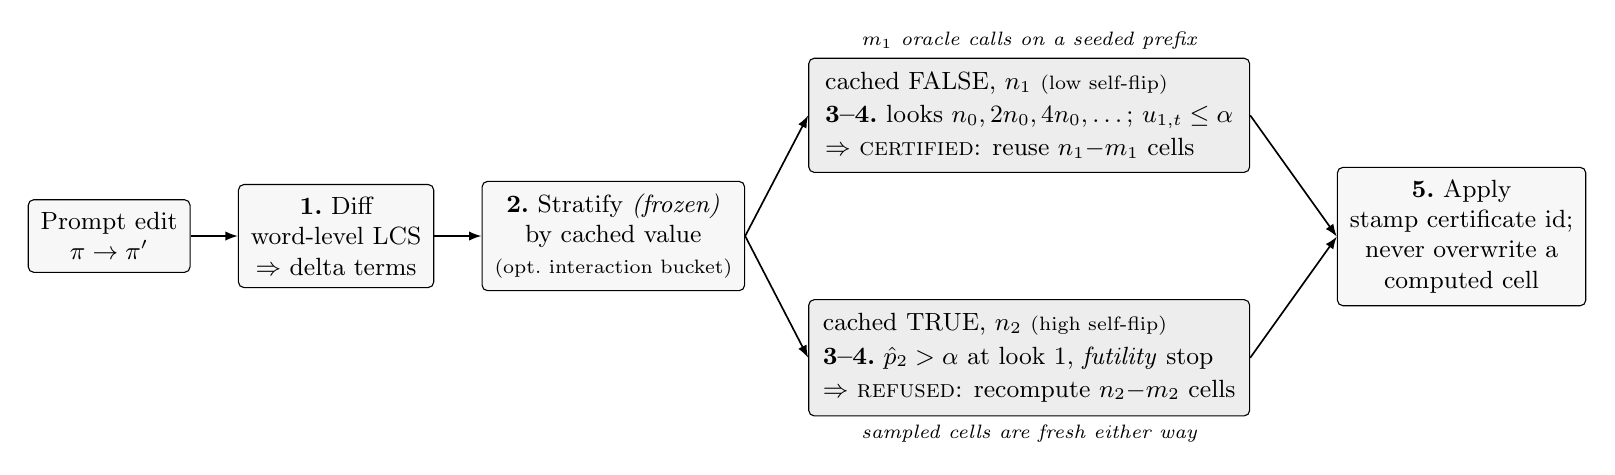
\begin{tikzpicture}[
  font=\small,
  node distance=6mm,
  bx/.style={draw, rounded corners=2pt, align=center, inner sep=4.5pt,
             minimum height=9mm, fill=black!3},
  lane/.style={draw, rounded corners=2pt, align=left, inner sep=5pt,
               minimum height=13mm, minimum width=56mm, fill=black!7},
  ar/.style={-{Latex[length=4.5pt]}, semithick},
  lbl/.style={font=\scriptsize\itshape, inner sep=1.5pt},
]
\node[bx, minimum width=20mm] (edit) {Prompt edit\\$\pi \to \pi'$};
\node[bx, right=of edit, minimum width=22mm] (diff)
  {\textbf{1.}~Diff\\word-level LCS\\$\Rightarrow$ delta terms};
\node[bx, right=of diff, minimum width=26mm] (strat)
  {\textbf{2.}~Stratify \emph{(frozen)}\\by cached value\\
   {\scriptsize(opt.\ interaction bucket)}};

\node[lane, above right=1mm and 8mm of strat] (laneF)
  {cached FALSE, $n_1$ {\scriptsize(low self-flip)}\\[1pt]
   \textbf{3--4.}~looks $n_0, 2n_0, 4n_0, \dots$;
   $u_{1,t} \le \alpha$\\[1pt]
   $\Rightarrow$ \textsc{certified}: reuse $n_1{-}m_1$ cells};
\node[lane, below right=1mm and 8mm of strat] (laneT)
  {cached TRUE, $n_2$ {\scriptsize(high self-flip)}\\[1pt]
   \textbf{3--4.}~$\hat{p}_2 > \alpha$ at look~1, \emph{futility} stop\\[1pt]
   $\Rightarrow$ \textsc{refused}: recompute $n_2{-}m_2$ cells};

\coordinate (mid) at ($(laneF.east)!0.5!(laneT.east)$);
\node[bx, anchor=west, minimum width=28mm] (apply) at ($(mid)+(11mm,0)$)
  {\textbf{5.}~Apply\\stamp certificate id;\\never overwrite a\\computed cell};

\draw[ar] (edit) -- (diff);
\draw[ar] (diff) -- (strat);
\draw[ar] (strat.east) -- (laneF.west);
\draw[ar] (strat.east) -- (laneT.west);
\draw[ar] (laneF.east) -- (apply.west);
\draw[ar] (laneT.east) -- (apply.west);

\node[lbl, above=0.5mm of laneF] {$m_1$ oracle calls on a seeded prefix};
\node[lbl, below=0.5mm of laneT] {sampled cells are fresh either way};
\end{tikzpicture}}
\caption{The procedure on the configuration our experiments pin.
Stratification is frozen before any oracle call, so it moves power
but never validity (Assumption~\ref{as:frozen}); only steps 3--4 spend
model calls, and they stop on evidence about a stratum's \emph{rate},
which is independent of the stratum's size. The two lanes are the
outcome we measure throughout: the stable stratum certifies and is
reused under a certificate, while the volatile one is refused at every
budget we tried and recomputed. A refusal is a stability diagnosis of
that slice of the column (\secref{sec:problem}), reached at the cost of
one look instead of a full recomputation.}
\Description{Left-to-right flow diagram. A prompt edit feeds a diff
step, which feeds a frozen stratification step. The stratification
branches into two lanes, a cached-FALSE lane with low self-flip and a
cached-TRUE lane with high self-flip. Each lane runs the adaptive
look schedule; the FALSE lane's empirical-Bernstein bound clears the
budget and is certified for reuse, while the TRUE lane stops for
futility and is refused and recomputed. Both branches converge on an
apply step that stamps a certificate identifier on the reused cells,
adding values without overwriting any cell already computed at the new
version.}
\label{fig:procedure}
\end{figure*}

Given the edit $\pi\to\pi'$ and cached cells for the affected rows
(Figure~\ref{fig:procedure}):
\begin{enumerate}
\item \textbf{Diff.} Compute a word-level longest-common-subsequence (LCS) diff of the
prompts;
collect content terms of added/removed spans (the \emph{delta}).
\item \textbf{Stratify (frozen).} Partition rows by cached value. We
adopt the skeleton of proxy-certified selection~\cite{supg} deliberately
here: with a binary proxy this step is their reduction,
transported from one-shot selection to maintenance. What we change is
the guarantee it carries, from one aggregate bound over the selected set
to a bound per stratum, which is the only difference
\secref{sec:experiments} (B2$'$) isolates and the only one that
protects a subgroup whose floor differs from the column's.
Optionally refine each value stratum by an interaction bucket (lexical
delta-term overlap or embedding cosine between the delta text and the
row's bound content, tertile-bucketed): a validity-free refinement
that pays only when within-value flip risk is heterogeneous, and
otherwise costs power through the $\delta/K$ split
(\secref{sec:experiments}).
\item \textbf{Schedule.} For stratum $j$ of size $n_j$, fix a doubling
look schedule $L_j = (45, 90, 180, \dots)$ capped at $n_j$ and sized so
the final look can certify a zero-flip stratum; split the stratum's
error budget $\delta_j = \delta/K$ evenly across looks.
\item \textbf{Sample and test.} Draw the stratum's seeded shuffle once.
At each look $t$, reveal fresh draws for the prefix, compute the
Maurer--Pontil~\cite{maurer} empirical-Bernstein upper confidence bound
$u_{j,t}$ on the stratum flip rate at level $\delta_j/|L_j|$;
\emph{certify and stop} if $u_{j,t} \le \alpha$; \emph{stop for
futility} if the empirical rate alone exceeds $\alpha$.
\item \textbf{Apply.} Reuse all unsampled rows of certified strata
(recording certificate provenance per cell); recompute the rest.
Sampled rows are already fresh.
\end{enumerate}

\begin{theorem}[Validity under peeking]\label{thm:valid}
Let $K$ be the number of strata produced by the frozen stratifier and
$\delta_j = \delta/K$. Under
Assumptions~\ref{as:pin}--\ref{as:sample}, with probability at least
$1-\delta$ over sampling and oracle draws, every certified stratum $j$
has true flip rate $p_j \le \alpha$; consequently
$\mathrm{FR}^{\mathrm{pres}}_j \le \alpha$ in expectation for every
certified stratum and every union of certified strata (the empty
certification is vacuously valid). In reuse-set mode, where
certification at sample size $m_j$ requires
$u_{j,t} \le \alpha\,(n_j{-}m_j)/n_j$, the same event further implies
$\mathbb{E}\,\mathrm{FR}^{\mathrm{reuse}}_j \le \alpha$ for every
certified stratum.
\end{theorem}
\begin{proof}[Proof sketch]
Fix stratum $j$ with $p_j > \alpha$ (resp.\
$p_j > \alpha(n_j{-}m_j)/n_j$ at every look, in reuse-set mode).
Certifying requires some look $t$ whose empirical-Bernstein upper bound
falls below the true rate, an event of probability at most
$\delta_j/|L_j|$ per look; union bounds over the $|L_j|$ looks and $K$
strata give $\delta$. The futility rule only stops sampling, never
certifies, so it cannot increase the error probability. On the good
event: the expected presented-cells error of stratum $j$ is at most its
whole-stratum rate $p_j \le \alpha$, and any size-weighted union of
certified strata inherits the bound. For reuse-set mode, total expected
flips in the stratum are $n_j p_j \le n_j \alpha (n_j{-}m_j)/n_j$,
and at worst all of them fall in the remainder, so the remainder mean
is at most $\alpha$ in expectation. Sampling within a stratum is a uniform
without-replacement draw, while the empirical-Bernstein bound we apply
is stated for i.i.d.\ draws. We do not prove that the i.i.d.\ bound
dominates in this regime, and Assumption~\ref{as:sample} carries that
gap explicitly; sampling fractions in our pinned runs reach
\sampleFracHi, well outside any small-fraction argument.
Finite-population and betting
bounds~\cite{bardenet,wsr} are the principled replacement, and
\secref{sec:experiments} measures both inside the same pinned procedure:
a betting confidence sequence is tighter on this workload and certifies
more configurations (\boundBetConfigs\ against \boundEbConfigs\ in the
main seeded run), while the without-replacement bound performs on par
with Maurer--Pontil (\boundWorConfigs). Our betting construction is the
i.i.d.\ hedged capital process; it purchases power, not
without-replacement validity, so the gap this
assumption names stays open. A recent ablation of nine bound families
for selective prediction under risk control catalogues the same kind of
regime dependence~\cite{boundablation}. Closing this gap
properly means either proving the i.i.d.\ bound sufficient in this
regime or paying that power cost, and we do neither here. Our
calibration study (\secref{sec:experiments}) measures the procedure as
deployed, at every budget at which the paper reports a certification
($\alpha \in \{\calAlphaGrid\}$) and with
\calTightNulls\ configurations planted just above the budget, and finds
no unsafe certification across \calTrials\ trials. That is evidence for
the regimes we ran, not a proof for all of them.
\end{proof}

\paragraph{Power.} A clean stratum certifies at the zero-flip minimum
$n^{*}(\alpha,\delta') = \lceil 7\ln(2/\delta')/(3\alpha)\rceil + 1$
(the variance term vanishes), e.g.\ \minZeroFlipSample\ at $\alpha{=}0.05$ under the pinned
procedure ($K{=}2$, six looks). That is the \emph{fixed-plan} minimum,
and the doubling schedule cannot stop on it: the first look at or above
$n^{*}$ is the one it takes, so a clean stratum actually pays
\minZeroFlipRealized\ draws in calibration. Either way, savings require
strata much larger than $n^{*}$, i.e.\ large tables, which is precisely
the deployment regime. Near the frontier, certifying a stratum with true
rate $p$ requires roughly
$n \gtrsim \tfrac{2p(1-p)\ln(2/\delta')}{(\alpha-p)^2}$ samples, which
explains the measured collapse of savings as $\alpha \downarrow p$
(Table~\ref{tab:main}, Stack Overflow (SO) formatting: \frontierA\ $\to$ \frontierB\ $\to$
\frontierC\ mean savings $\to$ refusal as $\alpha$ tightens $0.2 \to 0.02$).

\section{Implementation}
\label{sec:impl}

\sivm{} runs inside \emph{lore}, a working AI-table system: a
natural-language search bar compiles to a
versioned filter specification executed identically on MySQL and
Elasticsearch (conformance-tested for count, page, sort, aggregation,
and hydration parity on \corpusSO\ rows); AI columns are per-cell jobs
with typed structured outputs, bounded concurrency, retry, and a
content-hash cache keyed on \emph{only the bound fields}
$\beta(\pi)$, so unrelated row changes never invalidate the cache and
content-duplicate rows share one computation. Every run passes a
pre-run cost gate and lands in a ledger; prompt edits create
immutable versions (the \sivm{} substrate); certificates persist with
full strata evidence, and reused cells carry visible provenance in the
UI. Decode is pinned ($T{=}0$) for all cell computation per
Assumption~\ref{as:pin}.

\paragraph{Storage model.} Cells are keyed by
(column, row, prompt version), so versions of a column \emph{coexist}
instead of replacing one another, and a secondary index on
(column, version, model, content hash) serves the cache. This is the one
design decision \sivm{} actually depends on. Systems that key a cell by
row alone, or that hash the prompt into the cache key, destroy the old
materialization at the moment of the edit, and the question this paper
asks cannot then be posed: there is nothing left to certify. Keeping
versions side by side turns ``which cached cells still transfer?'' into
a join between two versions of one table, which is why the certifier is
a query over the store, not a service beside it.

\paragraph{Certificates are records, not decisions.} A certificate
persists the budget $\alpha$, the prompt delta, the per-stratum evidence
(size, cells sampled, bound attained, certified or refused), and the
sampled, reused, and recompute counts. It is therefore auditable after
the fact: the realized-error audits in \secref{sec:experiments} are
recomputed from the certificate's own persisted reuse set by a script
that shares no code with the certifier. Applying a certificate is a
single \texttt{INSERT\,\dots\,SELECT} that carries certified values
forward under the new version and stamps the certificate identifier on
each one.

That insert carries an anti-join against the target version, so reuse is
strictly \emph{additive}: a certificate can supply a value where none
was computed, and can never overwrite one that was. An earlier
implementation used an upsert, which is the obvious way to write it and
is silently destructive: applying a certificate
after a partial recompute reverted freshly computed cells to the stale
values the certificate had been asked to reuse. The bug is invisible in
aggregate error, because a reverted cell and a reused cell are the same
row with the same value; it surfaces only if something outside the
certifier knows what that cell should have said. Any system that
maintains stochastic cells across versions has this hazard, and the
guard belongs in the write path, not in code review.

\section{Experiments}
\label{sec:experiments}

\begin{table*}[t]
\centering
\caption{The pinned primary procedure (cached-value strata; adaptive
doubling looks $n_0{=}45$, six looks; $\delta{=}0.1$; presented-cells
estimand) on all five edit pairs, $n{=}\benchN$ each at temperature 0.
FR$_{\text{pres}}$/FR$_{\text{reuse}}$ are realized false-reuse over
presented cells and over the reuse set alone for the main seed; savings
(with 95\% percentile intervals) and certification rate are over
$B{=}\bootB$ sampling replications on frozen ground-truth labels; the
reuse-set violation rate is \emph{conditional on certifying}, i.e.\ its
denominator is the replications that issued a certificate, not $B$;
FR$_{\text{reuse}}$ carries a Wilson interval.
Reuse-set violation rates are $0.0\%$ in every configuration except SO
formatting at $\alpha{=}0.05$, a frontier-straddling cell discussed
below. The table is generated mechanically from the result files;
earlier exploratory sweeps with other stratifiers and schedules are
reported as ablations, not headline numbers.}
\label{tab:main}
\footnotesize
\input{\paperroot/table1}
\end{table*}

\paragraph{Baselines.} Three comparisons isolate what \sivm{} adds.
\emph{(B1) Verified-cache similarity has no cross-version signal:} the
per-row similarity between the v1-bound and v2-bound prompts, the
quantity a verified semantic cache thresholds, predicts cell flips at chance
as measured by the area under the receiver-operating-characteristic
curve (AUC \aucVcacheF\ formatting, \aucVcacheW\ widening; on the
formatting edit the score's entire range is \simLo--\simHi, because
shared row text dominates). Adding
``a version key'' to such a cache therefore cannot produce a sound
cross-version policy. Our interaction score carries real signal
exactly when the edit is semantic (AUC \aucInterW\ on widening) and
none above chance when flips are noise-driven (AUC \aucInterF\ on
formatting), which is why
the cached-\emph{value} dimension of stratification carries the
formatting case. \emph{(B2) Aggregate-only certification (no strata)}, run with the
\emph{same} schedule and budgets as the pinned procedure, is valid for
its aggregate estimand and silently corrupts subgroups. On the
formatting edit it \aggTightCertF\ at $\alpha{=}0.1$
(\aggFtSavings\ savings, \aggFtRealized\ aggregate error) while the
reused cached-TRUE subgroup carries \aggFtSubgroup\ error, and at
$\alpha{=}0.2$ it certifies \aggFsavings\ at \aggFrealized\ aggregate
with \aggFsubgroup\ subgroup error; on the widening edit it
\aggTightCertW\ at $\alpha{=}0.1$ and certifies \aggWsavings\ at
$\alpha{=}0.2$ with \aggWsubgroup\ subgroup error. Per-stratum bounds
are what make the guarantee mean something for every user-visible slice
of the table, and the effect is not an artifact of giving the baseline a
shorter schedule. \emph{(B2$'$) A SUPG-style competitor, matched.} The closest existing
method is proxy-certified selection~\cite{supg}: score rows with a cheap
proxy, spend an oracle budget labeling a sample, threshold the proxy so
the selected set's error clears the target. We transported it to
maintenance with the proxy the reduction in \secref{sec:system} names,
the cached value itself, and matched it to \sivm{} on every axis we
could: identical oracle budget, identical labels, identical error
target, the same total error budget $\delta$, each
split across the number of tests its own procedure performs (\sivm{}
across strata and looks, $\hhSivmPerTest$ per test; the competitor
across its candidate thresholds, $\hhValuePerTest$), and the same
reported quantity (error among reused cells, not the presented-cells
rate \sivm{} certifies).

Matched this way it is a live competitor that wins on volume and loses
on where its errors land. At $\alpha{=}0.2$ on the formatting edit it
reused \hhSupgReused\ cells to \sivm{}'s \hhSivmReused\ from the same
\hhBudget\ labels, and at \hhSupgErr\ realized error it satisfies the
bound it was given, against \sivm{}'s \hhSivmErr. On the widening edit
the same pattern: \hhSupgReusedW\ reuses at \hhSupgErrW\ versus
\hhSivmReusedW\ at \hhSivmErrW. The extra volume is drawn from the
volatile stratum, \hhSupgTrueRows\ cached-TRUE cells on the formatting
edit and \hhSupgTrueRowsW\ on the widening edit, where the per-stratum
floor is \floorTrueStratum\ and no aggregate target can make reuse safe;
\sivm{} reuses none of them. \secref{sec:problem} predicts this
behavior: an aggregate target
is satisfied by any mixture that averages out, so it buys volume with
the correctness of the least stable subgroup, and per-stratum bounds
are what extend the guarantee to that part of the table.

With
the cached value as the proxy there are only three candidate
thresholds, and at $\alpha{=}0.2$ the aggregate bound clears at the
loosest one, so the arm selects \hhSupgSelFrac\ of the rows it was
allowed to on the formatting edit and \hhSupgSelFracW\ on the widening
edit. Matched this way, the competitor reduces to B3, reuse everything,
with a certificate attached: its bound is satisfied, its aggregate
error is real, and its behavior is indistinguishable from the
guarantee-free status quo. The difference \sivm{} makes here is that
per-stratum bounds refuse a subgroup an aggregate target is willing to
spend.

We note two caveats on the same experiment. First,
run with an embedding-interaction proxy instead of the cached value the
reduction names, and with its much larger threshold search corrected
accordingly, the competitor certifies nothing at any budget we tried: a
proxy that does not separate flipping rows from stable ones cannot be
rescued by the selection procedure wrapped around it, which is what our
own stratifier ablation teaches from the other direction. Second, the
competitor's per-test level is looser than \sivm{}'s because it runs
fewer tests, and its volume advantage is sensitive to that: the
comparison is matched on the quantity a user sets ($\delta$ in total),
not on the level of any individual test, and we report both so the
reader can see which one the result rests on.

\emph{(B3) Guarantee-free embedding transfer}
(GPTCache-style~\cite{gptcache}, $\tau{=}0.95$) reuses every cell on the
formatting edit and \bThreeReuseW\ of them on the widening edit,
silently absorbing error at roughly the population flip rates
(\flipSoFormatting; \flipSoWidening): the
deployed status quo. That $\tau$ sits on the shoulder of the widening
edit's collapse, quantified in the threshold sweep below.

\paragraph{Setup and evaluation protocol.} All cells use one
budget-class reasoning model (DeepSeek V4 Flash, accessed through a
single gateway) at temperature zero; every ground-truth pass, sample, and
replay is seeded and reproducible from released scripts. Flip labels come
from single fresh draws under the new version, which matches the estimand
(a label answers ``would a recompute differ from the cache now?''). A
three-draw relabeling of the headline pair quantifies the instrument's
own variance: with fresh labels on
both sides the edit flips \editFlipFreshBoth\ of cells, versus
\floorBoolStored\ when only the v2 side is drawn fresh against the
frozen evaluation vector, and \floorBoolVote\ under majority-vote
labels; \labelChurn\ of rows relabel between instruments. That
\floorBoolStored\ is the same population quantity Table~\ref{tab:main}
reports as \flipSoFormatting\ for this edit, measured on the same
\benchN\ rows with a different v2 draw; the two differ by
\flipInstrumentGapRows\ rows, which is what single-draw labeling
costs, and we report the churn instead of picking whichever instrument
flatters the result. (The within-version floor, \floorBool, is
the separate quantity that bounds certifiability.) Labels are individually noisy with about a point of
draw-to-draw spread in the aggregate, which the replication standard
deviations in Table~\ref{tab:main} dominate, and it is population
functionals, not labels, that the guarantee addresses. Ledgered model spend across every experiment in this paper is
\totalSpend\ for \totalCells\ billed cells, read from the system's own
cost ledger. That figure is a lower bound, not a total: the ledger
records only cells written through the column runner, and a further
\offLedgerCells\ cells were computed by probe scripts that call the
model directly (the self-flip probes, the vote-of-3 study, the
multi-draw relabeling, and the second-model replication).

\paragraph{Noise floors and the stability law.} Replicate self-runs give
the two columns' intrinsic self-flip rates. The boolean column's floor
is \floorBool, measured from within-version draw pairs over $n{=}\benchN$
rows (an initial $n{=}200$ two-draw probe read \floorTzeroProbe\ and is
superseded); the
4-way select's floor is \floorSelect\ ($n{=}200$ probe; every observed
self-flip was between adjacent tiers). At default temperature the boolean
floor rises to \floorDefaultT\ on that same $n{=}200$ probe, whose
$T{=}0$ arm read \floorTzeroProbe: the claim rests on the
within-instrument contrast, and the default-temperature floor alone
exceeds a $5\%$ budget, which motivates decode pinning. Formatting-only
edit flip rates sit above each floor (\flipSoFormatting\ over
\floorBool; \flipDjFormatting\ over \floorSelect): on the boolean
column formatting flips are floor-dominated, and on both columns
instability scales with task hardness, not edit semantics
(the Djinni criteria change lands at \flipDjCriteria,
indistinguishable from its formatting edit).

\paragraph{A second model family.} Every measurement above uses one
model, so we replicated the three load-bearing quantities on a second,
weaker model from a different family (\texttt{\altModelName},
$n{=}\altModelN$ rows of the same evaluation vector, same prompts, same
$T{=}0$). Its self-flip floor is \altModelFloor: seven times
our primary model's \floorBool, and above every error budget a
user would plausibly set. The formatting edit flips \altModelEditFlip\
of its cells, again barely above its own floor, and the certifier
refuses every stratum at $\alpha{\in}\{0.1, 0.2\}$ after
90 oracle calls. This is the floor prediction of \secref{sec:problem}
operating as specified: a model that cannot reproduce its own answers
cannot support certified reuse at any budget, and the procedure detects
that cheaply instead of certifying something unsafe. \sivm{}'s value is
therefore a function of the
model's self-consistency, which is measurable before any edit is made,
and the same futility machinery that refuses semantic edits refuses
unstable models.

\paragraph{Main results.} Table~\ref{tab:main} reads as follows. On the
stable boolean column, the certifier reuses aggressively where safe
(formatting at $\alpha{\ge}0.1$; \benchSavings\ savings, interval
\benchSavingsPi, at $\alpha{=}0.2$ with realized presented-error
\benchRealized\ and a reuse-set rate whose Wilson interval is
\benchRealizedCi) and refuses semantic edits at tight
budgets; on the unstable select column, it certifies only at
$\alpha{=}0.2$ and correctly treats formatting and criteria edits alike.
Only \certifyingConfigs\ of the \tableConfigs\ default-mode
configurations in Table~\ref{tab:main} certify in any replication:
budgets below a
stratum's intrinsic rate are refused, and the refusals are the frontier
of Figure~\ref{fig:frontier}, not failures of the procedure.
No unsafe stratum was certified in any
seeded run, in \bootB\ sampling replications of every configuration, or in
the calibration study below; realized presented-cells error stayed
within $\alpha$ throughout. One frontier cell shows nonzero
reuse-set-metric exceedance, printed in Table~\ref{tab:main}:
conditional on certifying at all, which it does in \edgeCertRate\ of
replications at $\alpha{=}0.05$, the reuse-set metric exceeds $\alpha$
in \edgeExceed\ of those. This does not violate $\delta$, which bounds
the certification event, not that metric; nor is it covered by
Theorem~1, whose reuse-set guarantee applies only to certifications
made in reuse-set mode, and run in that mode this cell never certifies.
The strict reuse-set mode, whose deflated threshold shrinks with
sampling depth, prices the stronger guarantee, and the price varies
widely across the grid. On the headline edit at $\alpha{=}0.2$ it is
nearly free: \reuseSetSavingsMain\ savings against \benchSavings, still
certifying in essentially every replication. One budget tighter it
collapses, to \reuseSetSavingsTight\ savings certified in
\reuseSetCertTight\ of replications, and on the unstable select column
it never certifies reliably: no Djinni configuration at any budget
certifies in more than \reuseSetDjCertMax\ of replications.
Guaranteeing the stale subset alone is therefore affordable exactly
where the column is stable and the budget is loose, and unaffordable
everywhere else.

\begin{figure}[t]
\centering
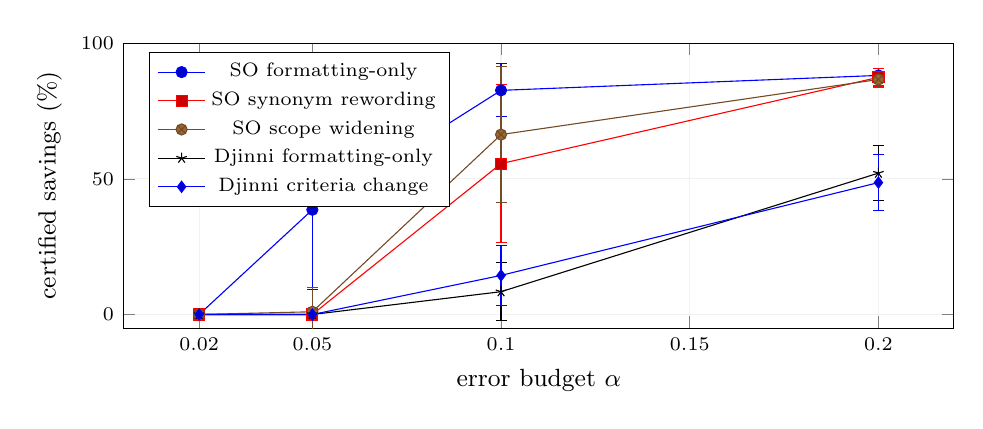
\begin{tikzpicture}
\begin{axis}[width=\linewidth, height=5.2cm, xlabel={error budget $\alpha$},
  ylabel={certified savings (\%)}, xmin=0, xmax=0.22, ymin=-5, ymax=100,
  label style={font=\small}, tick label style={font=\scriptsize},
  xtick={0.02,0.05,0.1,0.15,0.2},
  xticklabel style={/pgf/number format/fixed},
  legend pos=north west, legend style={font=\scriptsize}, grid=major,
  grid style={opacity=0.2}]
\frontierplots
\end{axis}
\end{tikzpicture}
\caption{The $\alpha$-savings frontier under the pinned procedure: mean
$\pm$ sd over \bootB\ sampling replications per point, generated from the
result files. Savings collapse as $\alpha$ approaches each column's
intrinsic flip rate.}
\Description{Line plot of certified savings against the error budget
alpha for five prompt-edit pairs. All curves start at zero savings at
the tightest budget and rise steeply as alpha loosens, with the two
Djinni curves rising far later and far less than the three Stack
Overflow curves.}
\label{fig:frontier}
\end{figure}

\begin{figure}[t]
\centering
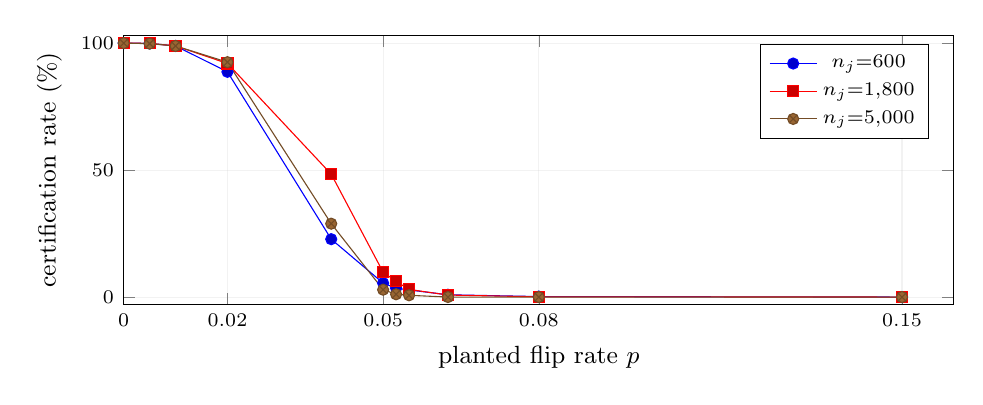
\begin{tikzpicture}
\begin{axis}[width=\linewidth, height=5cm, xlabel={planted flip rate $p$},
  ylabel={certification rate (\%)}, xmin=0, xmax=0.16, ymin=-3, ymax=103,
  label style={font=\small}, tick label style={font=\scriptsize},
  xtick={0,0.02,0.05,0.08,0.15},
  xticklabel style={/pgf/number format/fixed},
  legend pos=north east, legend style={font=\scriptsize}, grid=major,
  grid style={opacity=0.2}]
\powerplots
\end{axis}
\end{tikzpicture}
\caption{Calibration power at $\alpha{=}0.05$ (presented estimand,
$2{,}000$ trials per point): certification rises
smoothly as $p$ falls below $\alpha$, and is zero for every
$p > \alpha$ (no unsafe certifications in any calibration trial). Power
saturates once a stratum exceeds what the schedule can sample: the
$n_j{=}1800$ and $n_j{=}5000$ curves coincide because the six-look
schedule caps both at the same sample size.}
\Description{Line plot of certification rate against the planted flip
rate for three stratum sizes. Every curve certifies always when the
planted rate is zero, falls to never before the planted rate reaches
the budget, and stays there above it; the two larger stratum sizes
trace the same curve.}
\label{fig:power}
\end{figure}

\paragraph{The $\alpha$-frontier and adaptive economics.}
(Figure~\ref{fig:frontier}.) Savings collapse
as $\alpha$ approaches a stratum's intrinsic rate, exactly as the power
analysis predicts; below the floor the certifier refuses. The doubling
schedule prices both directions: uncertifiable edits are refused after
90 oracle calls, whereas a fixed plan pays the full zero-flip minimum,
and near-frontier certifications escalate sampling only while the data
stays consistent with certifiability.

\paragraph{Deployment scale.} To test the claim that sample cost is
table-size-independent, we materialized the boolean column across the
\emph{entire} \deployN-row corpus: \deployMatCells\ billed cells in a
single ledgered run costing \deployMatCost\ at \perCellCost\ per cell
(the remaining \deployFreeRows\ rows cost nothing, served by
content-hash caching or already materialized by earlier passes),
and \deployMatHours\ hours of model time reconstructed from the stored
per-cell latencies at \deployConcurrency-way concurrency. We then
certified the formatting edit against that materialized column with the
real model as oracle. Provenance: the materialization
and the first certification pass were live; the sweeps reported here are
a subsequent replay of the same seeded procedure against the stored
cells, which is also what a redundant certification would do in
production, so the wall-clock figures below are ledger-derived
model-time estimates; the replay itself was not timed. At $\alpha{=}0.2$ the procedure spent
\textbf{\deployOracle\ oracle calls} to certify reuse of
\textbf{\deployReused\ cells}, refusing the \deployTrueStratum-row
cached-TRUE stratum and so recomputing the \deployRecompute\ of its
cells that the futility stop had not already drawn fresh. That count is
one draw from an adaptive schedule, and an unremarkable one:
replicating the same
procedure over \bootB\ resamplings of the benchmark column puts the
budget at \benchOracleMean\ calls on average with median
\benchOracleMedian\ and range \benchOracleRange, so the deployment run
landed exactly on that distribution's median. A deployment should
budget for the upper end of that range, not either central value,
since the schedule stops on evidence and a near-frontier stratum
escalates. Either way the conclusion is unchanged: \deploySavings\ fewer model calls
(\deployMaintCells\ calls against \deployN), against a ceiling of
\deployCeiling\ set by the volatile cached-TRUE stratum that the
certifier never certifies: at this budget the procedure captures
essentially all of the reuse that is available to capture, and the
residue is a property of the column, not of the method. Priced at the ledger's
measured \perCellCost\ per cell, that maintenance workload would cost
\deployMaintCost\ and about \deployMaintMinutes\ minutes of model time,
against the \deployMatCost\ and \deployMatHours\ hours the corpus
actually cost to materialize. We do not quote a decision latency: the
only wall clock we hold for these sweeps is the replay's own
(\deployReplayMs\ ms at $\alpha{=}0.2$), which measures reading stored
cells, not issuing the oracle calls a live decision would pay
for, and is therefore not a figure any deployment could use. The run also applied the certificate,
persisting a \texttt{reuse\_certificate} row and stamping
its identifier on \deployStamped\ of the \deployReused\ reused cells,
which is what the table then serves and what the interface marks as
reused. The \deployUnstamped\ it does not stamp are exactly the audited
rows already recomputed for ground truth, because the apply step refuses
to write over a cell that already holds a freshly computed value at the
new version: a certificate can add a reused value but can never revert a
recomputation. We price the recompute leg without executing it: the
certifier identified those
\deployRecompute\ cells, and we did not spend a second corpus
materialization recomputing them. At
$\alpha{=}0.1$ the schedule escalated to \deployOracleTight\ calls for
\deploySavingsTight\ savings.

The comparison to the $n{=}\benchN$ benchmark run shows that sampling
cost did not scale with $n$: at $\alpha{=}0.2$ the
budget was drawn from the same distribution at both scales
(\benchOracleRange\ calls, mean \benchOracleMean, against \benchN\
rows; \deployOracle\ against \deployN), because
the doubling schedule stops on evidence about a stratum's \emph{rate},
which is size-independent, not on its size. The budget is not
deterministic, though: a schedule stops at the first look whose bound
clears $\alpha$, so the realized count is a draw, and the two budgets
show opposite faces of that. At $\alpha{=}0.2$ the runs stopped at
different looks, \benchOracleMain\ calls on the benchmark against
\deployOracle\ at deployment scale: respectively the minimum and the
median of the same \benchOracleRange\ replication distribution, which is
the spread an adaptive schedule is supposed to have. At $\alpha{=}0.1$ they stopped at
the \emph{same} look, \benchOracleTight\ calls each, which is the
maximum of that budget's replication distribution (mean
\benchOracleTightMean, median \benchOracleTightMedian, range
\benchOracleTightRange): a budget close to the stratum's own flip rate
drives many replications to that maximum, and both observed runs landed
there. The scaling itself held: sampling cost is $O(1)$ in
$n$ while the certifiable population is $O(n)$, so savings rose from
\benchSavingsMain\ to \deploySavings\ on the comparable single-run
measurement (\benchSavings\ is the benchmark's \bootB-replication mean,
quoted elsewhere; mixing the two would attribute part of the gain to an
estimator change instead of to scale).

Realized error was audited against oracle-computed v2 labels only
(status \texttt{done}/\texttt{cached}; certificate copies are excluded
by construction, as verbatim v1 values would register as non-flips):
\deployRealized\ over \deployOverlap\ audited reused rows, of which
\deployAuditReleased\ belong to the released $n{=}\benchN$ evaluation
vector and show \deployAuditReleasedErr\ on their own. That subset is
most of the audit and carries the same labels as the benchmark row of
Table~\ref{tab:main}, so it is a consistency check, not
independent evidence; the genuinely independent portion is the
remainder, audited against oracle cells outside the released vector. A separate
verifier script recomputes this audit from the run's persisted reuse-set
row identifiers and reproduces both figures exactly. Both are inside
both budgets. One reproducibility caveat: in MySQL the projection
list changes which rows a seeded \texttt{ORDER BY RAND} returns, so the
evaluation sample is defined by an exact query string, not by the seed
alone.

\paragraph{The stratification hierarchy.} Aggregate-only certification
(one stratum) is valid for its aggregate estimand yet conceals up to
\aggFtSubgroup\ realized error in the reused cached-TRUE subgroup: it
buys its aggregate with the stratum whose floor is \floorTrueStratum,
which per-value strata quarantine by construction.
Refining further by embedding-interaction tertiles helps only when
within-value risk is heterogeneous and otherwise
costs power through the $\delta/K$ split: on the headline
configuration the
value$\times$embedding-tertile refinement certifies strictly less than
value strata alone (\ablationSavings\ vs \benchSavings\ savings on SO
formatting at $\alpha{=}0.2$), because the split outweighs its
discrimination gain. Across all \ablationTotal\ shared configurations of
the released ablation the refinement is better in \ablationBetter\ and
worse in \ablationWorse, and the single win is a fraction of a point at
a budget where both stratifiers certify essentially nothing. We report
this as a negative result instead of tuning until it inverts: the
refinement's validity is unconditional (Assumption~\ref{as:frozen}), its
power is not, and on these columns within-value risk is homogeneous
enough that the $\delta/K$ split is never repaid.

\paragraph{Minority-stratum anatomy.} The cached-TRUE stratum of the
boolean column flips \minoritySingle\ under a formatting edit; vote-of-3 on
both sides reduces this to \minorityVote\ and shows that \minorityNoise\ of cached TRUE
values were single-draw noise; the flips that survive vote-3 are
genuine boundary volatility. Quarantine-and-recompute is therefore the correct systemic
response, and the actionable upstream knob is vote-based computation of
boundary-stratum cells at write time.

\paragraph{Calibration.} (Figure~\ref{fig:power}.) With planted flip rates across
$p \in \calPRange$, budgets $\alpha \in \{\calAlphaGrid\}$ (including the
one every headline result uses), stratum sizes $\{600, 1800, 5000\}$,
both estimands, and \calConfigs\ configurations (\calTrials\ runs), the
procedure never certified any stratum with $p > \alpha$, and the
realized presented-cells error never exceeded $\alpha$ in any certified
run of either mode. \calTightNulls\ of those configurations are
\emph{tight} nulls, planted just above the budget at $1.05$ to $1.25$
times $\alpha$, where the futility rule cannot dispose of the stratum at
the first look and the sampling fraction climbs; the worst certification
rate over all of them is \calTightWorstCert. This is the regime that
probes Assumption~\ref{as:sample}, since a
without-replacement correction would matter only where the bound is
close to the truth. The reuse-set rate evaluated on presented-mode
certifications does fluctuate past $\alpha$ in rarely-certifying
frontier configurations (worst \calWorstReuseMetric\ of certified runs at
$p{=}\calWorstP$, $\alpha{=}\calWorstAlpha$, certified \calWorstCertRate\ of the time):
this is expected, since presented-mode does not certify that metric; running
the strict reuse-set mode drives it to zero everywhere, with certification power rising smoothly as $p$ falls below
$\alpha$ and with stratum size. The conservatism gap (realized violations
far below nominal $\delta$) is the known cost of Bonferroni composition;
it is not budget that can be reclaimed.

\paragraph{The bound is the binding constraint, not the procedure.} Every
result above spends its budget through a Maurer--Pontil bound split
across looks by Bonferroni. That choice, not the stratification or the
schedule, is what sets the frontier, and we measured how much by swapping
the bound inside the same pinned procedure over the same stored labels.
On a clean sample at $n{=}90$ the Maurer--Pontil bound reads
\boundEbAtN; a Waudby-Smith--Ramdas betting confidence sequence, which
is anytime-valid and therefore spends the stratum's budget without
splitting it across the six looks, reads \boundBetAtN; the
empirical-Bernstein--Serfling without-replacement bound reads
\boundWorAtN. End to end across the \boundConfigsTotal\ configurations
of Table~\ref{tab:main}, the betting sequence certifies
\boundBetConfigs\ of them against \boundEbConfigs\ in the main seeded
run (the count of \certifyingConfigs\ above admits any configuration
that certifies in at least one replication), raises mean savings
from \boundEbSavings\ to \boundBetSavings, and does it on
\boundBetOracle\ oracle calls against \boundEbOracle: more certificates,
more savings, and a third fewer calls, simultaneously. The widest single
gap is the scope-widening edit at $\alpha{=}0.1$, which goes from
\boundGapEbSavings\ savings for \boundGapEbOracle\ calls to
\boundGapBetSavings\ for \boundGapBetOracle. The without-replacement
bound certifies \boundWorConfigs\ configurations, on par with
Maurer--Pontil: discharging Assumption~\ref{as:sample} is roughly
free, but gains none of the sequence's power.

A tighter bound is usable only if it remains valid, so we check
validity first. Replaying the calibration protocol with the betting
sequence substituted, over \boundCalTrials\ trials, no null
configuration's certification rate is demonstrably above $\delta$: the
worst is \boundBetNullWorst\ against a per-stratum $\delta$ of $0.05$,
and \boundBetNullsOver\ of \boundNullConfigs\ null configurations have a 95\% confidence interval lying entirely
above it. Maurer--Pontil certifies no null configuration in that same
replay: the conservative bound leaves almost all of its error budget
unspent, and a clean stratum costs it \boundEbCleanSample\ draws where
the sequence needs \boundBetCleanSample. We report this as an ablation
and leave the procedure pinned as run, because the headline results
and the deployment run were certified under Maurer--Pontil, and
restating every number under a bound the paper did not run would
misattribute the deployment evidence. The
frontier in Figure~\ref{fig:frontier} is therefore a property of the
bound, and implementations of \sivm{} should adopt the betting
sequence.

\paragraph{Embedding-transfer operating points.} A measured $\tau$
sweep over per-row similarities shows the guarantee-free transfer
baseline collapses within a $\approx 0.02$-wide threshold window
(formatting: \tauFmid\ of rows reused at $\tau{=}0.96$, \tauFhi\ at
$0.98$, none at $0.99$; widening: \tauWmid\ at $0.94$, \tauWhi\ at
$0.96$, none at $0.97$), and, decisively, realized error among reused
rows stays at the population flip rate at every operating point
(\tauFerrLo--\tauFerrHi\ and \tauWerrLo--\tauWerrHi): the threshold controls volume,
never error, because cross-version similarity carries no per-cell flip
signal (B1).

\section{The prompt-edit benchmark}
\label{sec:benchmark}

Semantic benchmarks exist, but they benchmark \emph{engines} on a fixed
task~\cite{sembench}; none exercises maintenance across prompt versions,
which needs a different artifact: version pairs plus per-cell flip labels
against the new version. Ours comprises: two redistributable corpora (Stack Overflow Developer
Survey, \corpusSO\ rows, ODbL~1.0/DbCL~1.0; Djinni English candidate
profiles, \corpusDjinni\ rows, MIT); three materialized columns of two
types (two boolean columns over structured facets, one of them the
production column and one a lab replica seeded from its second version;
one 4-way ordinal select over long free text); five realistic edit
pairs spanning formatting-only, synonym rewording, scope widening, and
criteria change; full ground-truth flip labels for $n{=}\benchN$ rows
per version pair at pinned decode (\labeledCells+ labeled cells), plus
self-flip replicate labels for both columns; and the deterministic
harness (seeded sampling, adaptive certifier, baseline policies) that
reproduces every number in this paper. Ledgered model spend across the
entire evaluation is \totalSpend\ (plus \offLedgerCells\ cells from
direct-call probes the ledger does not see), so the benchmark is cheap
to extend to new models.

\section{Related work}
\label{sec:related}

\paragraph{Guaranteed semantic query processing.} Semantic-operator
systems bound the error of \emph{one-shot} execution against a gold
model: LOTUS's optimized operators with accuracy targets~\cite{lotus},
SUPG's proxy-based selection with precision/recall
guarantees~\cite{supg}, BARGAIN's adaptive cascade
thresholds~\cite{bargain}, ThalamusDB's approximate natural-language predicates with
error bounds~\cite{thalamusdb}, and pipeline-level accuracy budgeting
in Task Cascades~\cite{taskcascades}. All certify a \emph{fixed}
definition per query; none transfers evidence across a definition
change. We reuse their statistical machinery (sampling, empirical-Bernstein bounds,
cascade framing) in a maintenance loop those systems do not model.

\paragraph{Verified caching.} vCache certifies that a \emph{new query}
may reuse a cached answer under one fixed definition, with learned
per-entry thresholds and user error rates~\cite{vcache}; Evergreen
spends confidence sequences and early stopping to cut the cost of
\emph{verifying} semantic aggregates, not to decide
reuse~\cite{evergreen}; and FreshCache approves a cache hit only when a
learned staleness model puts the probability that the entry is stale
below a per-tier error budget~\cite{freshcache}. FreshCache is the
closest in shape, since a per-partition budget gating reuse is exactly
our skeleton, and it differs on the two axes that decide the guarantee:
its risk is change-of-\emph{world} (open-web evidence ageing under fixed
query semantics) where ours is change-of-\emph{definition}, and its
per-tier quantity is a fitted model's point estimate where ours is a
finite-sample upper confidence bound that either clears $\alpha$ or
refuses. Our B1 baseline
shows why these mechanisms do not port: across a definition change the
query-to-entry similarity that such caches threshold carries no
per-cell flip signal (AUC \aucVcacheF\ and \aucVcacheW). \sivm{} certifies
change-of-\emph{definition} transfer, the axis those systems hold
fixed; the two compose (a certificate is scoped to a snapshot, and
change-of-world machinery decides when the snapshot itself expires).

\paragraph{Incremental and adaptive view maintenance.} Sampling a stale
materialized view to bound the error of answers served from
it~\cite{svc} is the closest classical relative of what we do, and the
difference is what goes stale: there the data drifts under a fixed view
definition, here the definition itself changes over fixed data, which is
why their staleness estimators condition on updates and ours condition
on a prompt delta. Classical IVM and view adaptation after
redefinition~\cite{gupta95,dbsp} assume
deterministic operators, where a rewrite either preserves a
subexpression or does not. Stochastic LLM cells break the premise: our
measurements show that even a semantically null rewrite flips cells at a
rate above the column's noise floor (\flipSoFormatting\ against
\floorBool), so ``preserved'' is not a property a rewrite can have here,
only a rate one can bound. Streaming semantic systems recompile
operators mid-stream but recompute outputs instead of certifying reuse
of old ones~\cite{vectraflow,contprompts}, and streaming cascades
certify on the \emph{data-arrival} axis, where new tuples meet a fixed
operator, and leave the definition axis open~\cite{streamcascades}.
Given that distinction,
\sivm{} is, to our knowledge, the first
maintenance procedure whose unit of transfer is a
\emph{statistically certified set of stochastic cells}.

The nearest counterexample shape is step-level reuse with lightweight
verification and selective patching across perturbed
requests~\cite{stepcache}, which does reuse computation when a request
changes. It differs on exactly the property this paper is about: its
verification is a deterministic per-step check, so it carries no error
budget and makes no population statement about the set it reuses.
In-database prompt management~\cite{promptdb} and versioned,
provenance-tracked prompt views~\cite{spear} supply the substrate this
work assumes, not a competing mechanism; we take the framing of
prompts as versioned views from that line and claim only the
certification machinery built on top of it, whose reuse is of
\emph{outputs}, not of KV state.

\paragraph{Prompt sensitivity and regression.} Prompt-delta analysis
for assertion synthesis~\cite{spade} anticipates our edit taxonomy but
targets pipeline quality checks, not reuse certification; interactive
LLM regression tools frame migration pain without
guarantees~\cite{retain}. Our finding that surface edit class does not
predict flip rate (synonym $\approx$ semantic; formatting $\approx$
floor-dominated) shows why measurement, not taxonomy, must
carry the decision.

\section{Limitations and outlook}
\label{sec:limits}

Bonferroni across strata and looks is sound but conservative, and
\secref{sec:experiments} prices that conservatism instead of
asserting it: a betting confidence sequence lifts mean certified savings
from \boundEbSavings\ to \boundBetSavings\ on a third fewer oracle
calls, at a null certification rate that stays inside $\delta$.
Adopting it is the largest power upgrade we measured; e-value selection
(e-BH)~\cite{ebh} composes with it. It is not a soundness
upgrade: the betting construction is i.i.d., so the
without-replacement gap in Assumption~\ref{as:sample} stays open, and
the Serfling-corrected bound that closes it performs on par with
Maurer--Pontil on this grid, so soundness and the sequence's power
gains do not yet combine. Our stratifiers are first instances; the
lexical variant is weak on broad edits, and the embedding variant's
signal exists only for semantic edits, so learned interaction models
are an open lever with guaranteed validity
(Assumption~\ref{as:frozen}). Equivalence is exact-match; free-text
columns need a judge whose own error must be calibrated and folded
into $\alpha$. Measurements use one budget-class
reasoning model for the full experimental program and a second, weaker
family only for the floor and refusal check; the quantitative frontier
(where savings sit for a given $\alpha$) is therefore
model-specific, even though the qualitative structure, a measurable
floor that bounds certifiability, held on both. Certificates are scoped to pinned
snapshots and say nothing about provider drift; composing \sivm{} with
change-of-world invalidation~\cite{evergreen,freshcache} is natural
future work. Finally, the economic frame that matters in production is
time-to-consistency under provider rate limits, where certified maintenance samples
\sampleFracLo--\sampleFracHi\ of cells across the reliably-certifying configurations of
Table~\ref{tab:main} (\sampleFracLo\ on the headline formatting edit at
$\alpha{=}0.2$) instead of recomputing $100\%$, a wall-clock and
rate-limit gain that grows with table size, because sample sizes do
not.

\section{Conclusion}
\label{sec:conclusion}

Prompt-defined columns are materialized views whose \emph{definition}
changes far more often than their data, and the systems serving them
today choose between recomputing everything and reusing everything.
\sivm{} shows the middle is reachable and cheap: freeze a
stratification, sample on a doubling schedule, bound each stratum's flip
rate, reuse only what clears the budget. At deployment scale that cost
\deployOracle\ oracle calls to certify reuse of \deployReused\ of
\deployN\ cells, and the sample did not have to grow with the table,
because the schedule stops on evidence about a \emph{rate}, which is
size-independent.

The result we did not anticipate is that the certifier doubles as a
measuring instrument for the column it maintains. A stratum refused at
every budget is a slice of the table on which the model cannot
reproduce its own answers, identified by a futility stop at the cost of
one look. Certified maintenance is therefore useful even where it
certifies nothing: the refusal identifies, cheaply, reuse error that
would otherwise go unmeasured.

\section*{Availability and reproducibility}
The system, the certifier, every experiment script, and every result
artifact are prepared for deposit as a single archive; the archive URL
will be added to this paper when it is public.
Released: the two corpora (already public and redistributable
under ODbL~1.0/DbCL~1.0 and MIT), the five versioned edit pairs, the
per-cell ground-truth flip labels, the certifier, the adapter
conformance suite, and every script and result artifact that produces a
number in this paper. Both corpora are used as distributed by their
maintainers under those licenses; the Djinni corpus is released
anonymized at source, and this work collects no new human-subject
data, attempts no re-identification, and releases only per-cell labels
and aggregate statistics. Withheld until the archive is public: nothing in
the evaluation path. Anyone reproducing this needs a model endpoint of
their own; the labels are released so the statistical results can be
reproduced without one. Several numbers here (the per-stratum floors,
the ledger economics, the materialization wall clock, the certificate's
stamp count) are computed from the running system's database, not
from a result file, so the generator dumps every one of those database
reads to an artifact alongside the others; the release is therefore
self-contained, with no dependence on our instance. Every quantitative claim in this
paper's prose, tables, and figures is emitted by a single generator
(\texttt{scripts/experiments/gen-paper-assets.ts}) from those artifacts
and from the system's cost ledger, and cited through macros, never
typed inline, so re-running an experiment regenerates the sentences that
cite it. This is enforced mechanically:
\texttt{scripts/check-paper-numbers.ts} fails on any of nine
conditions: (1) a hand-typed quantity in the prose outside an
enumerated allow-list (user parameters such as $\alpha$ and $\delta$,
protocol constants such as the schedule looks, and generic thresholds
quoted as such); (2) a quantity hardcoded inside the generator instead
of derived from an artifact; (3) a macro defined but never cited, since
an uncited macro can drift undetected; (4) a macro whose trailing space
is swallowed into the next word, which is invisible in the source;
(5) a sentence that asserts two quantities differ while citing two
macros whose values are equal, which is how an earlier draft printed
``different looks'' beside a number repeated twice; (6) a spelled-out
multiplier (``twice'', ``an order of magnitude'') that the cited
macros' ratio does not support, which is how a rate $1.26$ times a
floor was printed as double it; (7) a containment claim (``inside'',
``at most'') that the cited range and scalar macros do not support;
(8) an absolute claim (``never'', ``every'', ``anywhere'') appearing in
the abstract or the contributions list without an entry in an
enumerated allow-list, the one class of defect the numeric guards are
blind to by construction; and (9) a scope claim (``on the same
column'') whose cited macros come from different columns, checked
against a provenance file the generator emits from the same pair
definitions the experiments run on. It reports zero of all nine for
this draft. Each guard exists because the
corresponding defect reached a compiled PDF at least once, several of
them in a draft whose numbers were already machine-generated: generating
the quantities is necessary but not sufficient, because the sentences
that \emph{relate} quantities go stale independently of the quantities
themselves. Two reproducibility hazards we hit
are documented in the harness: seeded \texttt{ORDER BY RAND} in MySQL
depends on the projection list, so evaluation samples are pinned by
exact query string; and naive linear-congruential PRNGs written with
JavaScript number multiplication silently lose low bits, so all
sampling uses exact 32-bit arithmetic.


%% References are ACM Reference Format, as PVLDB requires. Entries live in
%% refs.bib and carry only citations confirmed by the verification audit in
%% docs/research/verification-verdict.md.
\bibliographystyle{ACM-Reference-Format}
\bibliography{refs}

\end{document}

